\documentclass[serif, aspectratio=169]{beamer}
\usepackage[T1]{fontenc} 
\usepackage{fourier}
\usepackage{hyperref}
\usepackage{latexsym,amsmath,xcolor,multicol,booktabs,calligra}
\usepackage{graphicx,pstricks,listings,stackengine}
\usepackage{listings}

\author{Dr.Hajialiasgari}
\title{Machine Learning}
\institute{
    Tehran University \\
    Of\\
    Medical Science
}
\date{\small \today}
\usepackage{UoWstyle}

% Define custom colors and styles for listings
\definecolor{deepblue}{rgb}{0,0,0.5}
\definecolor{deepred}{RGB}{153,0,0}
\definecolor{deepgreen}{rgb}{0,0.5,0}
\definecolor{halfgray}{gray}{0.55}

\lstset{
    basicstyle=\ttfamily\small,
    keywordstyle=\bfseries\color{deepblue},
    emphstyle=\ttfamily\color{deepred},
    stringstyle=\color{deepgreen},
    numbers=left,
    numberstyle=\small\color{halfgray},
    rulesepcolor=\color{red!20!green!20!blue!20},
    frame=shadowbox,
}

\begin{document}

\begin{frame}
    \titlepage
    \vspace*{-0.6cm}
    \begin{figure}[htpb]
        \begin{center}
            \includegraphics[keepaspectratio, scale=0.05]{Tumsl-logo.png}
        \end{center}
    \end{figure}
\end{frame}

\begin{frame}    
\tableofcontents[sectionstyle=show, subsectionstyle=show/shaded/hide, subsubsectionstyle=show/shaded/hide]
\end{frame}

\section{What is Machine Learning?}
\begin{frame}{What is Machine Learning}
    \begin{itemize}
        \item Tom M. Mitchell defines machine learning in his book "Machine Learning" (1997) with a widely accepted and clear definition:
    \item “A computer program is said to learn from experience E with respect to some class of tasks T and performance measure P, if its performance at tasks inv T, as measured by P, improves with experience E.”
    \end{itemize}
\end{frame}

\begin{frame}
    \begin{itemize}
        \item Breaking Down the Definition:
        \item Task (T): The specific activity the program is designed to perform (e.g., recognizing handwritten digits, recommending movies, or cancer detection).
        \item Experience (E): The data or interactions that the program is exposed to during training.
        \item Performance Measure (P): A quantitative metric to evaluate how well the program performs the task.
    \end{itemize}
\end{frame}

\section{Different Types of Machine Learning}
\begin{frame}{Supervised Learning}
    \begin{itemize}
        \item In supervised learning, the model learns from labeled data, where each input (feature) is paired with a corresponding output (label or target). The goal is to learn a mapping from inputs to outputs.
        \item In other words, we provide the computer with the problem and its solution, enabling it to discover answers for unsolved problems.
    \end{itemize}
\end{frame}

\begin{frame}{Supervised Learning Example}
    \begin{itemize}
        \item \texttt{\color{orange}Regression:}Predict continuous values (e.g., house prices, temperature).
        \item \texttt{\color{orange}Classification:}Predict discrete categories (Heart Disease Detection,Classifying the risk level of cardiovascular diseases using patient vitals and medical history)
    \end{itemize}
\end{frame}

\begin{frame}
    \centering
    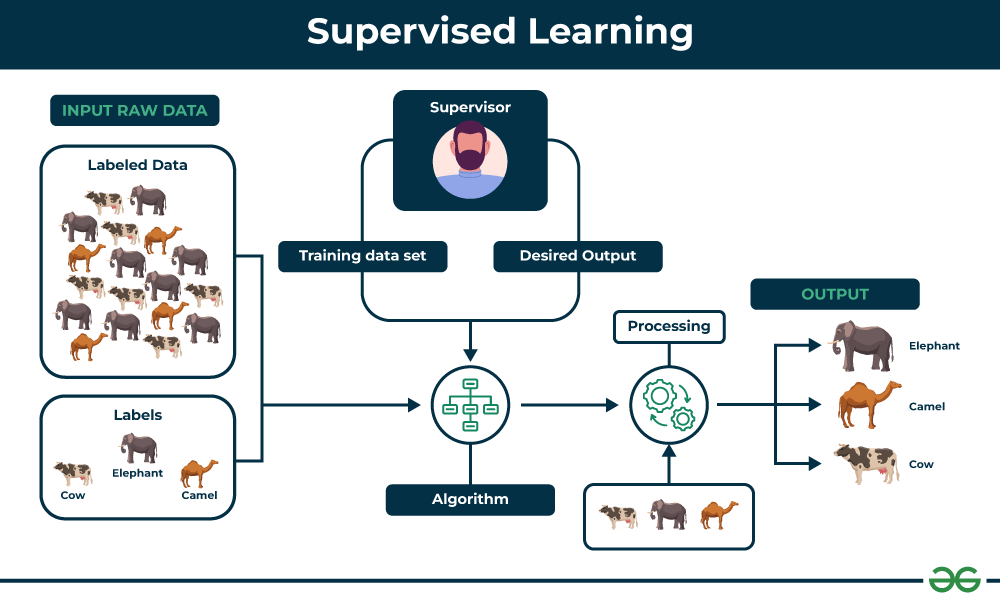
\includegraphics[width=0.8\textwidth]{supervised-learning.png}
\end{frame}

\begin{frame}{Unsupervised Learning}
    \begin{itemize}
        \item In unsupervised learning, the model learns patterns or structures from data without labeled outputs. It is used to uncover hidden patterns or groupings.
    \end{itemize}
\end{frame}

\begin{frame}{Unsupervised Learning Example}
    \begin{itemize}
        \item \texttt{\color{orange}Clustering:} Group similar data points (e.g., customer segmentation).
        \item Algorithms: K-Means, DBSCAN, Hierarchical Clustering.
    \end{itemize}
\end{frame}

\begin{frame}
    \centering
    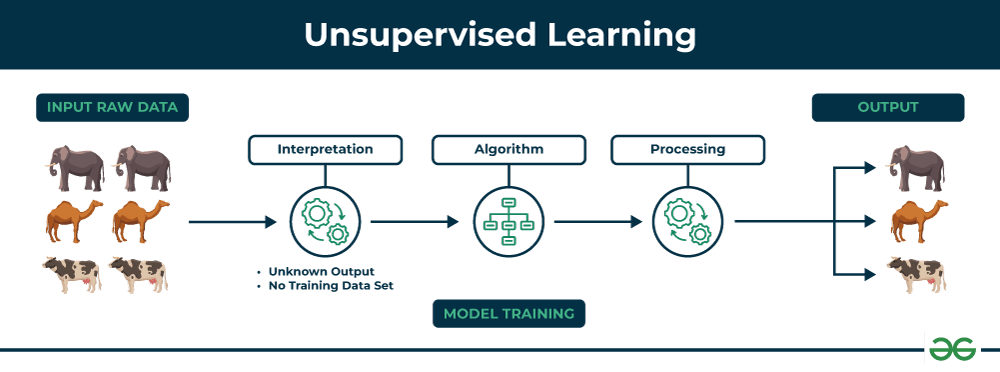
\includegraphics[width=0.8\textwidth]{Unsupervised-learning.png}
\end{frame}


\begin{frame}{Semi-Supervised Learning}
    \begin{itemize}
        \item Semi-supervised learning combines elements of supervised and unsupervised learning. It uses a small amount of labeled data and a large amount of unlabeled data to improve learning.
        \item Example : Image recognition tasks with few labeled images and many unlabeled images.
    \end{itemize}
\end{frame}

\begin{frame}{Semi-Supervised Learning}
    \centering
    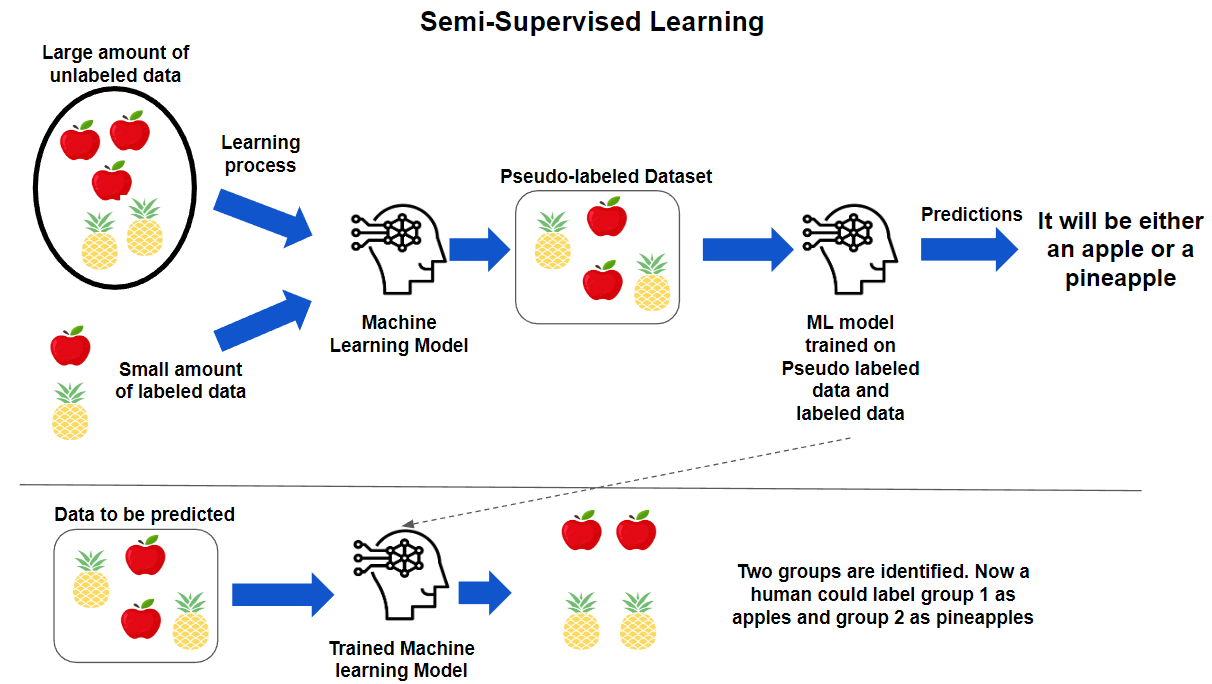
\includegraphics[width=0.8\textwidth]{semisupervised-learning.png}
\end{frame}

\begin{frame}{Reinforcement Learning}
    \begin{itemize}
        \item Reinforcement learning (RL) involves learning by interacting with an environment to achieve a goal. The model (agent) learns to take actions that maximize cumulative rewards.
        \item Example : Robotics, game playing (e.g., AlphaGo), autonomous vehicles.
    \end{itemize}
\end{frame}

\begin{frame}{Reinforcement Learning Components}
    \begin{itemize}
        \item Agent: The learner or decision-maker.
        \item Environment: The system the agent interacts with.
        \item Policy: A strategy that maps states to actions.
        \item Reward Signal: Feedback to guide learning.
    \end{itemize}
\end{frame}

\begin{frame}{Reinforcement Learning}
    \centering
    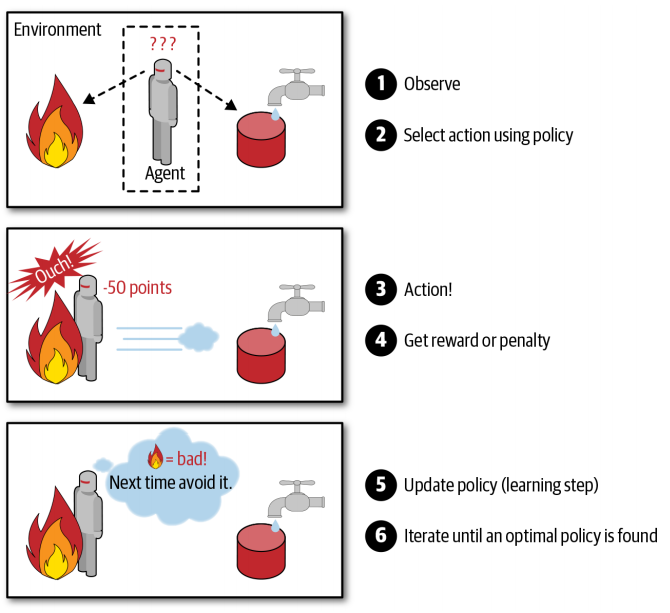
\includegraphics[width=0.7\textwidth, height=0.7\textheight]{RL.png}
\end{frame}

\begin{frame}
    \begin{center}
        {\Huge\ End of Preface}
    \end{center}
\end{frame}

\end{document}

